\documentclass{article}
\usepackage{geometry}
\usepackage{amsmath, amssymb, amsthm}
\usepackage{lmodern}
\usepackage{tikz}
\usetikzlibrary{positioning}

\usepackage[
backend=biber,
style=alphabetic,
sorting=ynt
]{biblatex}
\addbibresource{refs.bib}

\title{
\vspace{-2.5cm}
A research proposal for the computational complexity of
minimizing reducible sofic shifts
}
\author{Justin Cai}

\newcommand{\Ac}{\mathcal{A}}  % alphabet
\newcommand{\Fc}{\mathcal{F}}
\newcommand{\Lc}{\mathcal{L}}  % label function
\newcommand{\Gc}{\mathcal{G}}  % labeled graph
\newcommand{\Hc}{\mathcal{H}}  % labeled graph
\newcommand{\Vc}{\mathcal{V}}
\newcommand{\Ec}{\mathcal{E}}
\newcommand{\Bc}{\mathcal{B}}
\newcommand{\shift}[1]{\mathsf{X}_{#1}}
\newcommand{\term}[1]{\textit{#1}}
\newcommand{\co}{\mathsf{co}}
\newcommand{\GI}{\mathsf{GI}}

\newtheorem{theorem}{Theorem}
\newtheorem{definition}{Definition}
\newtheorem*{conjecture}{Conjecture}
% \newtheorem{example}{Example}

\begin{document}

\maketitle

\begin{abstract}
    In symbolic dynamics, a certain class of objects 
    called sofic shifts are sets of bi-infinite
    sequences that come from labeled graphs, such that each letter of 
    the sequence is the label of an edge in a bi-infinite walk around the graph.
    If one wanted to use sofic shifts to model something, it would be desirable to 
    have a graph that is as small as it can be while still presenting the same sequences.
    While the problem of how hard it is to compute this minimal graph for shifts with a 
    certain property called irreducibility is known, the hardness of computing the same
    problem for shifts that do not have this property is unknown.
\end{abstract}

\section{Background}

% Symbolic dynamics studies a class of bi-infinite sequences over a finite alphabet called 
% shift spaces; such spaces have the property of being shift invariant.

% A bi-infinite sequence over a finite alphabet \(\Ac\) is an assignment of a symbol
% from \(\Ac\) to each integer. Such sequences 

% In symbolic dynamics, the \term{full shift} \(\Ac^\mathbb{Z}\) is the collection of 
% all bi-infinite sequences over symbols from a finite alphabet \(\Ac\).
% Elements from the full shift are called a points. For a point \(x\) from the full shift,
% we can denote it \[x=(x_i)_{i \in \mathbb{Z}} = \hdots x_{-2} x_{-1} x_0 x_1 x_2 \hdots,\]
% where \(x_i\) is the \term{\(i\)th coordinate} of \(x\). Hence, a point is defined by assigning 
% each coordinate with a symbol from the alphabet.
% A \term{block}
% (or \term{word}) is a finite sequence of symbols from \(\Ac\). The block starting
% at the \(i\)th coordinate and ending at the \(j\)th coordinate
% is denoted \(x_{[i,j]}=x_i x_{i+1} \hdots x_{j}\). A block \(w\) \term{occurs} in \(x\)
% if there exists \(i,j \in \mathbb{Z}\) such that \(x_{[i,j]}=w\). For a collection
% of blocks \(\Fc\) over \(\Ac\), define \(\shift{\Fc}\) to be the subset of points in \(\Ac^\mathbb{Z}\) 
% such that every block in \(\Fc\) does not occur in \(x\). Finally, a \term{shift space} is a 
% subset \(X\) of the full shift such that there exists a collection \(\Fc\) such that \(X = \shift{\Fc}\).

% Let's look at some examples of shift spaces. For these examples, we'll consider sets 
% of sequences of Let \(X\) be the set of all 

A \term{full shift} is the set of all bi-infinite sequences over a finite alphabet \(\Ac\).
A \term{graph} \(G\) is a finite set of \term{vertices} \(\Vc=\Vc(G)\) and a finite set 
of edges \(\Ec = \Ec(G)\) with each edge \(e\) starting at a vertex \(i(e) \in \Vc\)
and terminating at a vertex \(t(e) \in \Vc\). 
A bi-infinite walk on \(G\) is a bi-infinite sequence of edges such that the 
terminating vertex of each edge is the inital vertex of the next edge. The set of 
all bi-infinite walks on \(G\) is called the \term{edge shift} \(\shift{G}\).
A \term{labeled graph} \(\Gc\)
is a graph \(G\) equipped with a \term{labeling} \(\Lc: \Ec(G) \to \Ac\), which assigns each
edge \(e\) from \(G\) a label \(\Lc(e)\) from a finite alphabet \(\Ac\). If \(x\) is 
a bi-infinite walk on \(G\), then the \term{label of the bi-infinite walk} \(\Lc_\infty(x)\) is 
the bi-infinite sequence of the labels of \(x\). The set of all labels of bi-infinite 
walks is called \term{presentation of \(\Gc\)}, denoted \(\shift{\Gc}\). A subset \(X\) of a full shift is a \term{sofic shift} if \(X = \shift{\Gc}\)
for some labeled graph \(\Gc\). A labeled graph \(\Gc\) is a \term{presentation} 
of \(X\) or \term{presents \(X\)} if \(X=\shift{\Gc}\).

For example, let \(X\) be the set of bi-infinite sequences over \(\{0,1\}\) such that 
there is an even number of \(0\)'s between any two \(1\)'s. Then \(X=\shift{\Gc}\), where
\(\Gc\) is any labeled graph in Figure 1. This shift is known as the \term{even shift}.
\begin{figure}[h]
    \centering
    \begin{tikzpicture}
        \node[shape=circle, draw=black] (A) at (0,0) {};
        \node[shape=circle, draw=black] (B) at (2,0) {};

        \path [->] (A) edge[out=225, in=135, distance=10mm] node[left] {$1$} (A);
        \path [->] (A) edge[out=45, in=135] node[above] {$0$} (B);
        \path [->] (B) edge[out=225, in=-45] node[below] {$0$} (A);

        \node[shape=circle, draw=black] (A) at (4,-1) {};
        \node[shape=circle, draw=black] (B) at (6,-1) {};
        \node[shape=circle, draw=black] (C) at (6,1) {};
        \node[shape=circle, draw=black] (D) at (4,1) {};

        \path[->] (A) edge[out=180, in=-90, distance=10mm] node[left] {$1$} (A);
        \path[->] (C) edge[out=0, in=90, distance=10mm] node[right] {$1$} (C);
        \path[->] (A) edge node[below] {$0$} (B);
        \path[->] (B) edge node[right] {$0$} (C);
        \path[->] (C) edge node[above] {$0$} (D);
        \path[->] (D) edge node[left] {$0$} (A);

        \node[shape=circle, draw=black] (A) at (8.5, 0) {};
        \node[shape=circle, draw=black] (B) at (10.5, -1) {};
        \node[shape=circle, draw=black] (C) at (10.5, 1) {};

        \path[->] (A) edge[out=135, in=-135, distance=10mm] node[left] {$1$} (A);
        \path[->] (A) edge node[below] {$1$} (B);
        \path[->] (B) edge[out=60, in=-60] node[right] {$0$} (C);
        \path[->] (C) edge[out=-120, in=120] node[left] {$0$} (B);
        \path[->] (C) edge node[above] {$0$} (A);

    \end{tikzpicture} 
    \caption{Presentations of the even shift}
\end{figure}

\newpage

A \term{block} is a finite sequence of symbols over an alphabet. Let \(x\) be a bi-infinite 
from a sofic shift. We say the a block \(w\) \term{occurs in} \(x\) if there exists 
integers \(i, j\) such that \(x_i x_{i+1} \hdots x_{j} = w\). The \term{language} of a 
sofic shift \(\Bc(X)\) is the collection of blocks that occur in any bi-infinite sequence in \(X\).
A sofic shift is \term{irreducible} if for any pair of blocks \(u,v \in \Bc(X)\), there 
exists another block \(w \in \Bc(X)\) such that \(uwv \in \Bc(X)\).

A presentation is \term{right-resolving} if for each vertex in the presentation, the 
labels of the outgoing edges of that vertex are all distinct. For example, the left and middle graphs 
in Figure 1 are right-resolving while the right graph is not right-resolving. A presentation  
is \term{irreducible} if for each pair of vertices in the graph, there exists a path in the graph 
from the first vertex to the second vertex and path from the second vertex to the first vertex.
A presentation that is not irreducible is \term{reducible}.
Each presentation in Figure 1 is irreducible, while the presentation in Figure 2 is reducible.

For a presentation \(\Gc\), the \term{follower set} of a vertex \(I\) is the labels of all 
(finite) paths that originiate from that vertex, denoted \(F_\Gc(I)\). The presentation is 
\term{follower-separated} if the follower sets of \(\Gc\) are distinct; that is,
for any pair of vertices \(I, J \in \Vc\) such that \(I \ne J\), then \(F_\Gc(I) \ne F_\Gc(J)\)

A \term{minimal} presentation of a sofic shift \(X\) is a presentation such that 
it has the fewest vertices among all presentations of \(X\); that is, 
a presentation \(\Gc\) is minimal for \(X\) such that for all 
presentations \(\Gc'\) of \(X\), \(|\Vc(\Gc)| \le |\Vc(\Gc')|\).

\section{Minimization of reducible presentations}


From \cite{lind1995introduction} corollary (3.3.20), given an irreducible right-resolving
presentation, we can find the minimal right-resolving presentation by merging 
vertices in the presentation that have the same follower set, creating a 
follower-seperated presentation. However, this does not work for reducible presentations, as 
being follower-separated does not imply minimality. We can see this with this presentation 
of the even shift:

\begin{figure}[h]
    \centering
    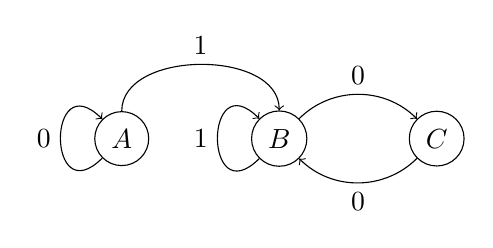
\begin{tikzpicture}
        \node[shape=circle, draw=black] (A) at (0,0) {\(B\)};
        \node[shape=circle, draw=black] (B) at (2,0) {\(C\)};
        \node[shape=circle, draw=black] (C) at (-2,0) {\(A\)};

        \path [->] (A) edge[out=225, in=135, distance=10mm] node[left] {$1$} (A);
        \path [->] (A) edge[out=45, in=135] node[above] {$0$} (B);
        \path [->] (B) edge[out=225, in=-45] node[below] {$0$} (A);
        \path [->] (C) edge[out=90, in=90] node[above] {$1$} (A);
        \path [->] (C) edge[out=225, in=135, distance=10mm] node[left] {$0$} (C);

    \end{tikzpicture} 
    \caption{A reducible, follower-separated presentation of the even shift}
\end{figure}

The block \(01\) does not appear in the follower set of \(B\), but does for the follower 
set of \(A\), so \(F_\Gc(A) \ne F_\Gc(B)\). The follower set of \(C\) is distinct from
the follower sets of \(A\) and \(B\), as any word that starts with \(1\) that appears in 
\(F_\Gc(A)\) and \(F_\Gc(B)\) does not appear in \(F_\Gc(C)\), so \(F_\Gc(A) \ne F_\Gc(C)\) and 
\(F_\Gc(B) \ne F_\Gc(C)\). Hence, the presentation is follower-separated. This graph also presents 
the even shift as any walk that visits \(A\) has a corresponding walk that only visits \(B\) 
and \(C\) (and the \(BC\) subgraph presents the even shift). Since this presentation is 
follower-separated, it would be minimized if (3.3.20) applied to reducible presentations, 
but since the graph presents the even shift, it is not minimal (as a minimal 
presentation of the even shift has 2 vertices).

Therefore, an algorithm for minimizing reducible presentations is still to be desired. However, 
a polynomial time algorithm might be unlikely, as this research conjectures that the problem 
of deciding if such presentation can be minimized is as hard as the graph isomorphism problem. 

The \(\GI\) complexity class is the set of decision 
problems that have a polynomial-time Turing reduction to the graph isomorphism problem (a 
\term{graph isomorphism} is an invertible mapping from the vertices of one graph 
to the vertices of another such that two vertices are connected if and only if they 
are connected under the isomorphism; the graph isomorphism problem asks given two 
graphs, decide whether there exists an isomorphism between the graphs).
Currently, it is unknown if \(\GI\) is contained in \(\mathsf{P}\) nor is \(\mathsf{NP}\)-complete \cite{kobler2012graph}.

Define the \term{minimal reducible presentation} problem, or \(\mathsf{minRP}\), as given a reducible presentation,
decide if it is a minimal presentation.
The complement problem \(\co\)-\(\mathsf{minRP}\) asks, given a reducible presentation, to decide if it is not minimal. 
A problem is \term{\(\GI\)-hard} if there exists a polynomial-time Turing reduction from 
any problem in \(\GI\) to that problem. Now, this research proposes the following 
conjecture:

\begin{conjecture}
    The complement of the minimal reducible presentation problem, \(\co\)-\(\mathsf{minRP}\), is \(\GI\)-hard.
\end{conjecture}

A reduction candidate I've looked at is to take two irreducible, minimal, right-resolving presentations 
that are isomorphic,
and then take an edge from one graph and change its terminal vertex to a vertex in the other graph, 
creating a reducible graph. For example, if we take two minimal presentations of the even shift,
we can connect them like so:

\begin{figure}[h]
    \centering
    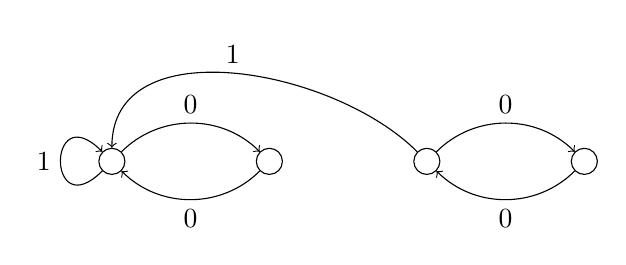
\begin{tikzpicture}
        \node[shape=circle, draw=black] (A) at (0,0) {};
        \node[shape=circle, draw=black] (B) at (2,0) {};

        \path [->] (A) edge[out=225, in=135, distance=10mm] node[left] {$1$} (A);
        \path [->] (A) edge[out=45, in=135] node[above] {$0$} (B);
        \path [->] (B) edge[out=225, in=-45] node[below] {$0$} (A);

        \node[shape=circle, draw=black] (C) at (4,0) {};
        \node[shape=circle, draw=black] (D) at (6,0) {};

        \path [->] (C) edge[out=135, in=90] node[above] {$1$} (A);
        \path [->] (C) edge[out=45, in=135] node[above] {$0$} (D);
        \path [->] (D) edge[out=225, in=-45] node[below] {$0$} (C);
    \end{tikzpicture}
    \caption{Connecting two even shifts to create a reducible, non-minimal even shift}
\end{figure}

The resulting graph still presents the even shift, so the presentation is not minimal.
Hence one could propose that two graphs are isomorphic if and only if there exists 
an edge in one graph and a vertex in the other such that if you connect them, then 
the resulting graph is not minimal.
For the reduction to hold, we'd still need to show that if two graphs are not 
isomorphic, then for any edge in one graph and any vertex in the other, the 
resulting graph from the connection is always minimal. However, there exists 
a counterexample:

\begin{figure}[h]
    \centering
    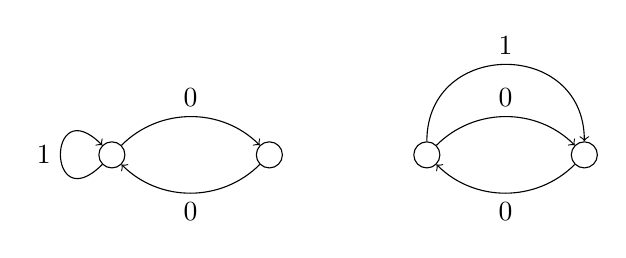
\begin{tikzpicture}
        \node[shape=circle, draw=black] (A) at (0,0) {};
        \node[shape=circle, draw=black] (B) at (2,0) {};

        \path [->] (A) edge[out=225, in=135, distance=10mm] node[left] {$1$} (A);
        \path [->] (A) edge[out=45, in=135] node[above] {$0$} (B);
        \path [->] (B) edge[out=225, in=-45] node[below] {$0$} (A);

        \node[shape=circle, draw=black] (A) at (4,0) {};
        \node[shape=circle, draw=black] (B) at (6,0) {};

        \path [->] (A) edge[out=45, in=135] node[above] {$0$} (B);
        \path [->] (B) edge[out=225, in=-45] node[below] {$0$} (A);
        \path [->] (A) edge[out=90, in=90, distance=13mm] node[above] {$1$} (B);
    \end{tikzpicture}
    \caption{Two non-ismorphic graphs that can be connected like Figure 3}
\end{figure}

You can take the edge labeled 1 on the right graph and connect it the same way as in Figure 3.
Thus, we have two graphs that are not isomorphic but there exists an edge and vertex such 
that the connected graph is not minimal. 

\newpage

Instead of modifying one of the graphs, one could augment the graphs by adding an 
edge with a label distinct to the labels of the two graphs from one of the graphs to 
the other and then adding a self loop with the same label on the vertex that was 
connected to. For example, starting again with two minimal even shifts,

\begin{figure}[h]
    \centering
    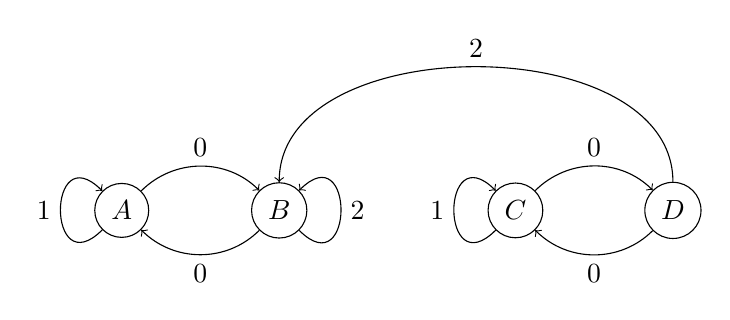
\begin{tikzpicture}
        \node[shape=circle, draw=black] (A) at (0,0) {\(A\)};
        \node[shape=circle, draw=black] (B) at (2,0) {\(B\)};

        \path [->] (A) edge[out=225, in=135, distance=10mm] node[left] {$1$} (A);
        \path [->] (A) edge[out=45, in=135] node[above] {$0$} (B);
        \path [->] (B) edge[out=225, in=-45] node[below] {$0$} (A);

        \node[shape=circle, draw=black] (C) at (5,0) {\(C\)};
        \node[shape=circle, draw=black] (D) at (7,0) {\(D\)};

        \path [->] (C) edge[out=225, in=135, distance=10mm] node[left] {$1$} (C);
        \path [->] (C) edge[out=45, in=135] node[above] {$0$} (D);
        \path [->] (D) edge[out=225, in=-45] node[below] {$0$} (C);

        \path [->] (D) edge[out=90, in=90] node[above] {$2$} (B);
        \path [->] (B) edge[out=-45, in=45, distance=10mm] node[right] {$2$} (B);
    \end{tikzpicture}
    \caption{A proposed reduction}
\end{figure}

The shift this graph presents is the same as the presentation of 
the subgraph consisting of vertex \(A\) and \(B\) and the edges
who begin in those vertices, as any walk that visits \(C\) and \(D\)
has a corresponding walk from the \(AB\) subgraph.


\printbibliography

\end{document}